\documentclass{article}
\usepackage[a4paper, total={7in, 10in}]{geometry}

\usepackage[utf8]{inputenc}
\usepackage{graphicx}
\usepackage{amsmath, amssymb}
\usepackage{empheq}
\usepackage{showlabels}
\usepackage{graphicx}
\graphicspath{ {./img_exercise/} }
\usepackage{float}  % In preamble

% Tiếng Việt
\usepackage[utf8]{vietnam}
% Chia nhiều cột trên trang
\usepackage{multicol}
% List
\usepackage{enumitem}


\begin{document}

\tableofcontents

\newpage
\section{Angles}
\begin{multicols}{2}

\subsection{Find the length of an arc of a circle of radius 5cm subtending a central angle measuring $\mathbf{15^o}$}
We have:
\begin{align*}
    &\theta = \frac{L}{r} \\
    &\rightarrow L = \theta r = \frac{15\pi 5}{180} = 1.31 cm
\end{align*}

\subsection{Find in degrees the angle subtended at the center of a circle of diameter 50 cm by an arc of length 11 cm}
We have (use with degree):
\begin{align*}
    &\theta = \frac{L}{r} = \frac{11}{50/2}.\frac{\pi}{180} = 25^o12'
\end{align*}

\subsection{In a circle of diameter 40 cm the length of a chord is 20 cm. Find the length of minor arc corresponding to the chord.}

\begin{figure}[H]
    \centering
    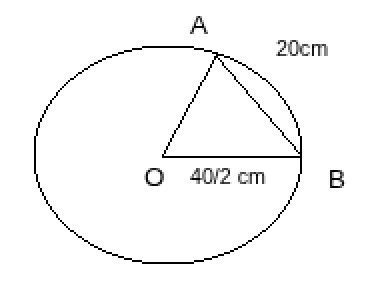
\includegraphics[width=0.25\textwidth]{begin-angles6.png}
\end{figure}

From formular we have
\begin{align*}
    &l = \frac{\pi r \theta}{180} \rightarrow \theta^o= \frac{l.180}{\pi r} \\
    &\theta = \frac{L}{r} \rightarrow L_{AB} = \frac{l.180}{\pi r}.\frac{\pi}{180}.r = 20cm
\end{align*}


\subsection{A horse is tied to a post by a rope, if the horse moves along a circular path always keeping the rope tight and describe 88 meters when it has traced out $\mathbf{72^o}$ at the center, find the length of the rope}

\begin{figure}[H]
    \centering
    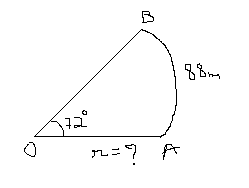
\includegraphics[width=0.25\textwidth]{begin-angles7.png}
\end{figure}

we have
\begin{align*}
    &l = \frac{\pi r \theta}{180} \rightarrow r= \frac{l.180}{\pi \theta^o} \\
    &r = \frac{88\times 180}{\pi.72} = 70.03 m
\end{align*}

\end{multicols}

\section{Trigonometry Ratio}

\begin{multicols}{2}

\subsection{If $\mathbf{\sqrt{3}\tan(\theta)=3\sin(\theta)}$, then find the value of $\mathbf{\sin^2(\theta)-\cos^2(\theta)}$ }

We have
\begin{align*}
    &\sqrt{3} \tan(\theta) = 3\sin(\theta) \rightarrow \frac{\tan(\theta)}{\sin(\theta)} = \frac{3}{\sqrt{3}} \\
    & \rightarrow \frac{1}{\sin(\theta)}.\frac{\sin(\theta)}{\cos(\theta)} = \frac{3}{\sqrt{3}} \rightarrow \frac{1}{\cos(\theta)} = \frac{3}{\sqrt{3}} \\
    & \rightarrow \theta = \cos^{-1}{\frac{\sqrt{3}}{3}} \\
    & \rightarrow \sin^2(\theta) - \cos^2(\theta) = \frac{1}{3}
\end{align*}

\subsection{In triangle ABC, right angled at B if $\sin A = 1/2$, find the value of \\
(a) $\sin C \cos A - \cos C \sin A$ \\
(b) $\cos A \cos C + \sin A \sin C$
}

\begin{figure}[H]
    \centering
    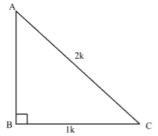
\includegraphics[width=0.2\textwidth]{expert-Tr2.png}
\end{figure}

\noindent $\sin A = BC/AC = 1/2. Set BC = 1k, AC = 2k.$ \\
So BA = $\sqrt{(2k)^2-k^2} = \sqrt{3k}$ \\
$\sin C = \frac{AB}{AC} = \frac{\sqrt{3}}{2} \quad \cos C=\frac{AB}{AC} = \frac{\sqrt{3}}{2}$ \\
$\cos A= \frac{AB}{AC} = \frac{\sqrt{3}}{2}$ \\
$(a) \sin C \cos A - \cos C \sin A $\\
\begin{align*}
    \frac{\sqrt{3}}{2}.\frac{\sqrt{3}}{2} - \frac{1}{2}.\frac{1}{2}= \frac{1}{2} 
\end{align*}
(b) $\cos A \cos C + \sin A \sin C$
\begin{align*}
    \frac{\sqrt{3}}{2}.\frac{1}{2} + \frac{1}{2}.\frac{\sqrt{3}}{2}= \frac{\sqrt{3}}{2} 
\end{align*}

\end{multicols}

\subsection{If $\mathbf{\theta}$ is an acute angle and $\mathbf{\frac{\sin\theta + 1}{\sin\theta + 1} = \frac{\sqrt{3}+2}{\sqrt{3}-2}}$}
\begin{align*}
    &\frac{\sin\theta \cos1 + \cos\theta \sin1}{\sin\theta \cos1 - \cos\theta \sin1} = \frac{\sqrt{3}+2}{\sqrt{3}-2} \\
    &\Big(\sin\theta \cos1 + \cos\theta \sin1\Big)\Big(\sqrt{3}-2\Big)=\Big(\sqrt{3}+2\Big)\Big(\sin\theta \cos1 - \cos\theta \sin1\Big) \\
    &\sqrt{3}\cos1\sin\theta + \sqrt{3}\sin1\cos\theta - 2\cos1\sin\theta - 2\sin1\cos\theta = \sqrt{3}\cos1\sin\theta - \sqrt{3}\sin1\cos\theta + 2\cos1\sin\theta - 2\sin1\cos\theta \\
    &\Big(\sqrt{3}\cos1 - 2\cos1\Big)\sin\theta + \Big(\sqrt{3}\sin1-2\sin1)\cos\theta = \Big(\sqrt{3}\cos1 + 2\cos1\Big)\sin\theta - \Big(\sqrt{3}\sin1 + 2\sin1\Big)\cos\theta \\
    & \Bigg[\Big(\sqrt{3}\cos1 - 2\cos1\Big)-\Big(\sqrt{3}\cos1+2\cos1\Big) \Bigg] \sin\theta = -\Bigg[\Big(\sqrt{3}\sin1 + 2\sin1 \Big) + \Big(\sqrt{3}\sin1 - 2\sin1\Big)\Bigg] \cos\theta \\
    & \text{We have:  } ax=by \rightarrow \frac{x}{y} = \frac{b}{a} \\
    &  \tan\theta = \frac{\sin\theta}{\cos\theta} = \frac{-\Big(\sqrt{3}\sin1 + 2\sin1\Big) - (\sqrt{3}\sin1 - 2\sin1 \Big)}{\Big(\sqrt{3}\cos1-2\cos1\Big) - \Big(\sqrt{3}\cos1 + 2\cos1\Big)} \\
    & \rightarrow \theta = 53^o26'
\end{align*}

\begin{multicols}{2}

\subsection{Find the height of the triangle}
\begin{figure}[H]
    \centering
    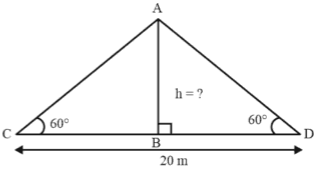
\includegraphics[width=0.3\textwidth]{expert-Tr4.png}
\end{figure}
We have
\begin{align*}
    &\tan(60) = \frac{h}{20/2} \\
    &\rightarrow h = \tan(60)*10 = 10\sqrt{3}
\end{align*}

\end{multicols}

\section{Trigonometry Angles}
\begin{multicols}{2}

\subsection{If $\mathbf{\sin(\theta)-\cos(\theta)=1}$, \\ then $\mathbf{\sin(\theta)\cos(\theta)}$ equal}
\begin{align*}
    &\frac{d}{h} - \frac{k}{h} = 1; \qquad \frac{d}{h}\frac{k}{h} = \frac{dk}{h^2} = ? \\
    &\frac{d}{h} = 1 + \frac{k}{h} \text{ and } \frac{k}{h}=\frac{d}{h}-1 \\
    &\sin\theta \cos\theta = \Big(1 + \frac{k}{h}\Big)\Big(\frac{d}{h}-1\Big) = ? \\
    &\frac{d}{h} - 1 + \frac{kd}{h^2} - \frac{k}{h} = ?\\
    &\frac{kd}{h^2}= \sin\theta \cos\theta = \frac{-d}{h} + \frac{k}{h}+1=-1+1=0
\end{align*}

\subsection{If $\mathbf{\sin(\theta) = e^x}$  \\ then $\mathbf{\cos(\theta)}$ equal}
\begin{align*}
    &\sin(\theta)=e^x \rightarrow \cos^2(\theta) + e^{2x} = 1 \\
    &\cos(\theta)= \sqrt{1-e^{2x}}
\end{align*}

\end{multicols}


\section{Trigonometry Formula}
\subsection{If $\mathbf{x = sec(\theta) + \tan(\theta)}$, then $\mathbf{x + \frac{1}{x}=?}$}
\begin{align*}
    x + \frac{1}{x} &= sec(\theta) + \tan(\theta) + \frac{1}{sec(\theta) + \tan(\theta)} \\
                    &= \frac{sec(\theta)\Big(sec(\theta) + \tan(\theta)\Big) + \tan(\theta)\Big(sec(\theta) + \tan(\theta)\Big) + 1}{sec(\theta) + \tan(\theta)} \\
                    &= sec^2(\theta) + sec(\theta)\tan(\theta) + \tan^2(\theta) +  sec(\theta)\tan(\theta) + 1 \\
                    &= sec^2(\theta) + sec(\theta)\tan(\theta) + \tan^2(\theta) +  sec(\theta)\tan(\theta) + sec^2(\theta) - \tan^2(\theta) \\
                    &= 2sec^2(\theta) + 2sec(\theta)\tan(\theta) \\
                    &= \frac{2sec(\theta)\Big(sec(\theta) + \tan(\theta)\Big)}{sec(\theta) + \tan(\theta)} \\
                    &= 2sec(\theta)
\end{align*}

\subsection{$\mathbf{\sqrt{\frac{1-\sin(\theta)}{1+\sin(\theta)}}}$ equal?}
\begin{align*}
    \sqrt{\frac{1-\sin(\theta)}{1+\sin(\theta)}} &= \sqrt{\frac{1-\sin(\theta)}{1+\sin(\theta)}} \times 1 = \sqrt{\frac{1-\sin(\theta)}{1+\sin(\theta)}} \times \sqrt{\frac{1-\sin(\theta)}{1 - \sin(\theta)}} \\
    &= \frac{\Big[1 - \sin(\theta) \Big]^{1/2} \times \Big[1 - \sin(\theta) \Big]^{1/2}}{\Big[1 + \sin(\theta) \Big]^{1/2} \times \Big[1 - \sin(\theta) \Big]^{1/2}} = \frac{1-\sin(\theta)}{\Bigg[\Big(1+\sin(\theta)\Big) \Big(1-\sin(\theta)\Big)\Bigg]^{1/2}} \\
    &= \frac{1-\sin(\theta)}{\Big[1-\sin(\theta)+\sin(\theta)-\sin^2(\theta) \Big]} \\
    &= \frac{1-\sin(\theta)}{\sqrt{1-\sin^2(\theta)}} = \frac{1-\sin(\theta)}{\sqrt{\cos^2(\theta)}} = \frac{1-\sin(\theta)}{\cos(\theta)} \\
    &= \frac{1}{\cos(\theta)} - \tan(\theta) = \sec(\theta) - \tan(\theta)
\end{align*}

\subsection{$\mathbf{\frac{\sin(\theta)}{1-\cot(\theta)} + \frac{\cos(\theta)}{1-\tan(\theta)}}$ equal?}
\begin{align*}
    \frac{\sin(\theta)}{1-\cot(\theta)} + \frac{\cos(\theta)}{1-\tan(\theta)} 
    &= \frac{\sin(\theta)[1-\tan(\theta)] + \cos(\theta)[1-\cot(\theta)]}{[1-\cot(\theta)][1-\tan(\theta)]} \\
    &= \frac{\sin(\theta)-\sin(\theta)\tan(\theta)+\cos(\theta)-cos(\theta)\cot(\theta)}{[1-\cot(\theta)][1-\tan(\theta)]} \\
    &= \frac{\sin(\theta)[1-\tan(\theta)] + \cos(\theta)[1-\cot(\theta))]}{[1-\cot(\theta)][1-\tan(\theta)]} \\
    &= \sin(\theta) + \cos(\theta)
\end{align*}

\section{Differentiation}
\begin{multicols}{2}

\subsection{$\mathbf{f(x)=6x^3-9x+4}$}
\begin{align*}
    f'(x)=18x^2-9
\end{align*}

\subsection{$\mathbf{f(x)=\sqrt{x} + 8\sqrt[3]{x}} - 2\sqrt[4]{x}$}
\begin{align*}
    f'(x) &= \frac{1}{2}x^{-1/2} + \frac{8}{3}x^{-2/3} - \frac{1}{2}x^{-3/4} \\
        &= \frac{1}{2\sqrt{x}} + \frac{8}{3\sqrt[3]{x^2}} - \frac{1}{2\sqrt[4]{x^3}}
\end{align*}

\subsection{$\mathbf{f(x)= 10\sqrt[5]{x^3} - \sqrt{x^7} + 6\sqrt[3]{x^8} - 3}$}
\begin{align*}
    f'(x) &= 6x^{-2/5} - \frac{7}{2}x^{5/2} + 16x^{5/3} \\
        &= \frac{6}{\sqrt{x^5}} - \frac{7\sqrt{x^5}}{2} + 16\sqrt[3]{x^5}
\end{align*}

\subsection{$\mathbf{g(x)=\frac{4x^3-7x+8}{x}}$}
Way 1: $(\frac{u}{v})^2 = \frac{u'.v - v'u}{v^2}$
\begin{align*}
    &u = 4x^3 - 7x + 8 \quad u' = 12x^2-7 \\
    &v = x            \quad v' = 1
\end{align*}
\begin{align*}
    g'(x) &= \frac{(12x^2-7)(x)-(4x^3-7x+8)}{x^2} \\
        &= \frac{12x^3 - 7x - 4x^3 + 7x - 8}{x^2} \\
        &= \frac{8x^3 - 8}{x^2} = \frac{8x^3}{x^2} - \frac{8}{x^2} = 8x - \frac{8}{x^2}
\end{align*}
Way 2:
\begin{align*}
    g(x) &= 4x^2 - 7 + 8x^{-1} \\
    g'(x) &= 8x - \frac{8}{x^2}
\end{align*}

\subsection{$\mathbf{y = e^{\sqrt{2x+17}}}$}
\noindent We have:
\begin{align*}
    (e^u)'=u'e^u \qquad  (\sqrt[n]{u})' = \frac{u'}{n\sqrt[n]{u^{n-1}}}
\end{align*}
So we have:
\begin{align*}
    \frac{dx}{dy} &= (\sqrt{2x+17})'e^{\sqrt{2x+17}} = \frac{2}{2\sqrt{2x+17}}e^{\sqrt{2x+17}} \\
                &=\frac{e^{\sqrt{2x+17}}}{\sqrt{2x+17}}
\end{align*}

\subsection{$\mathbf{y=e^x\ln(5x^3+x^2)}$}
\noindent We have:
\begin{align*}
    (uv)'=u'v +v'u \qquad (e^u)'=u'e^u \qquad (\ln(u))'=\frac{u'}{u}
\end{align*}
So,
\begin{align*}
    \frac{dy}{dx} = e^x\ln(5x^3+x^2) + \frac{(15x^2 + 2x)e^x}{5x^3 + x^2}
\end{align*}

\subsection{$\mathbf{y = \frac{x^2}{\ln(1-4x^2)}}$}
\noindent We have:
\begin{align*}
    \Big(\frac{u}{v}\Big)' = \frac{u'v-v'u}{u^2} \qquad (x^n)'= nx^{n-1} \qquad (\ln(u))'=\frac{u'}{u}
\end{align*}
So,
\begin{align*}
    \frac{dy}{dx} &= \frac{2x.\ln(1-4x^2)-\frac{-8x.x^2}{(1-4x^2)}}{\ln^2(1-4x^2)} \\
                &= \frac{2x(1-4x^2)\ln(1-4x^2)+8x^3}{(1-4x^2)\ln^2(1-4x^2)}
\end{align*}

\end{multicols}

\subsection{$\mathbf{y=\frac{\tan(x) + \cot(x)}{\tan(x)-\cot(x)}}$}
\noindent We have:
\begin{align*}
    \Big(\frac{u}{v}\Big)'=\frac{u'v-v'u}{v^2} \qquad (\tan(u))'=\frac{u'}{\cos^2(u)} \qquad (\cot(u))'=\frac{-u'}{\sin^2(u)}
\end{align*}
So, now we have
\begin{align*}
    \frac{dy}{dx} &= \frac{\Big(\frac{1}{\cos^2(x)} + \frac{-1}{\sin^2(x)}\Big)\Big(\tan(x)-\cot(x)\Big)-\Big(\frac{1}{\cos^2(x)} - \frac{-1}{\sin^2(x)}\Big)\Big(\tan(x)+\cot(x)\Big)}{\Big(\tan(x)-\cot(x)\Big)^2} \\
            &= \frac{\Big(\sec^2(x)-cosec^2(x)\Big)\Big(\tan(x)-\cot(x)\Big)-\Big(\sec^2(x)+cosec^2(x)\Big)\Big(\tan(x)+\cot(x)\Big)}{\Big(\tan(x)-\cot(x)\Big)^2} \\
            &= \frac{-2\tan(x)cosec^2(x)}{\Big(\tan(x)-\cot(x)\Big)^2}
\end{align*}

\begin{multicols}{2}

\subsection{Find $\mathbf{\frac{dy}{dx}} \text{ for } x^2+y^3=3$}
\noindent Differentiationg both size and aplly chain rule
\begin{align*}
    & \frac{dy}{dx}x^2 + \frac{dy}{dx}y^3 = \frac{dy}{dx}3\\
    &\rightarrow 2x + \frac{dy}{dx}3y^2 = 0\\
    &\rightarrow \frac{dy}{dx} = -\frac{2x}{3y^2}
\end{align*}

\subsection{Find $\mathbf{\frac{dy}{dx}} \text{ for } x^2+y^2=2$}
\noindent Differentiationg both size and aplly chain rule
\begin{align*}
    &(x^2+y^2=2)' \\
    &\rightarrow 2x+2y\frac{dy}{dx}=0 \\
    &\rightarrow \frac{dy}{dx} = \frac{-2x}{2y} = -\frac{x}{y}
\end{align*}

\subsection{Find $\mathbf{\frac{dy}{dx}} \text{ for } 2y^3+4x^2-y=x^6$}
\noindent Differentiationg both size and aplly chain rule
\begin{align*}
    &(2y^3+4x^2-y=x^6)' \\
    &\rightarrow 6y^2\frac{dy}{dx} +8x- \frac{dy}{dx}=6x^5 \\
    &\rightarrow \frac{dy}{dx} = \frac{-2x}{2y} = -\frac{x}{y}
\end{align*}

\subsection{Find $\mathbf{\frac{dy}{dx}} \text{ for } 7y^2+\sin(3x)=12-y^4$}
\noindent Differentiationg both size and aplly chain rule
\begin{align*}
    &(7y^2+\sin(3x)=12-y^4)' \\
    &\rightarrow 14y\frac{dy}{dx} + 3\cos(3x)=-4y^3\frac{dy}{dx} \\
    &\rightarrow \frac{dy}{dx}(14y+4y^3)=-3\cos(3x) \\
    &\rightarrow \frac{dy}{dx}= \frac{-3\cos(3x)}{14y+4y^3}
\end{align*}

\subsection{Find $\mathbf{\frac{dy}{dx}} \text{ for } xy=1$}
\noindent Apply product rule
\begin{align*}
    &(xy=1)' \\
    &\rightarrow x'y + xy' = 0 \\
    &\rightarrow \frac{dy}{dx}y = -x \\
    &\rightarrow \frac{dy}{dx}= -\frac{x}{y}
\end{align*}

\end{multicols}

\subsection{Find $y'$ for each of the follwing}
\textbf{a)} $x^3y^5 + 3x = 8y^3+1$ \\
\textbf{b)} $x^2\tan(y) + y^{10}\sec(x)=2x$ \\
\textbf{c)} $e^{2x+3y} = x^2 - \ln(xy^3)$ \\

\textbf{<Solution>} \par

\textbf{a)} $x^3y^5 + 3x = 8y^3+1$ \\
We have
\begin{align*}
    &(u.v)'=u'v+v'u \\
    &\rightarrow 3x^2y^5 + 5x^3y^4\frac{dx}{dy} + 3 = 24y^2\frac{dx}{dy} \\
    &\leftrightarrow \frac{dx}{dy}(5x^3y^4 - 24y^2) = -3 - 3x^2 + y^5 \\
    &\rightarrow \frac{dx}{dy} = \frac{-3 - 3x^2 + y^5}{5x^3y^4 - 24y^2}
\end{align*}

\end{document}